\documentclass[a4paper, 14pt]{extarticle}

\usepackage[
  left=20mm,
  right=10mm,
  top=20mm,
  bottom=20mm
]{geometry}

\usepackage{fontspec}
\setmainfont{Times New Roman}
\usepackage{unicode-math}
\setmathfont{XITSMath-Regular.otf}

\usepackage{polyglossia}
\setmainlanguage{russian}
\setotherlanguage{english}
\newfontfamily\cyrillicfont{Times New Roman}[Ligatures = TeX]
\usepackage{setspace}
\onehalfspacing
\setlength{\parindent}{1cm}

\tolerance=2000
\emergencystretch=3em
\hbadness=10000
\sloppy

\usepackage{fancyhdr}
\pagestyle{fancy}
\fancyhf{}
\fancyfoot[C]{\thepage}
\renewcommand{\headrulewidth}{0pt}

\usepackage{graphicx}
\usepackage{caption}

\DeclareCaptionLabelSeparator{gost}{~---~}
\captionsetup{
  labelsep=gost,
  font=normalsize
}

\captionsetup[table]{
  justification=raggedright,
  singlelinecheck=false,
  skip=6pt
}

\captionsetup[figure]{
  justification=centering
}

\usepackage{booktabs}
\usepackage{array}
\usepackage{amsmath}
\usepackage{float}

\usepackage{siunitx}
\sisetup{
  output-decimal-marker = {,},
  separate-uncertainty = true,
  exponent-product = \cdot
}

\usepackage{titlesec}
\titleformat{\section}[block]{\normalfont\bfseries}{\thesection}{1em}{}
\titlespacing{\section}{1cm}{*2}{*1.5}
\titleformat{\subsection}[block]{\normalfont\bfseries}{\thesubsection}{1em}{}
\titlespacing{\subsection}{1cm}{*2}{*1.5}
\titleformat{\subsubsection}[block]{\normalfont\bfseries}{\thesubsubsection}{1em}{}
\titlespacing{\subsubsection}{1cm}{*2}{*1.5}

\usepackage{enumitem}
\setlist{nosep}
\setlist[itemize,1]{label=---, leftmargin=1cm}
\setlist[enumerate,1]{label=\arabic*., leftmargin=1cm}

\usepackage{hyperref}
\hypersetup{
  colorlinks=false,
  hidelinks
}

\usepackage{tocloft}
\renewcommand{\cftsecleader}{\cftdotfill{\cftdotsep}}

\begin{document}

\thispagestyle{empty}

\begin{center}
  Министерство образования и науки Российской Федерации\\[0.5em]
  \textbf{НАЦИОНАЛЬНЫЙ ИССЛЕДОВАТЕЛЬСКИЙ}\\
  \textbf{ТОМСКИЙ ГОСУДАРСТВЕННЫЙ УНИВЕРСИТЕТ (НИ ТГУ)}\\[0.3em]
  Физический факультет\\

  \vspace{4cm}

  \textbf{\Large ЛАБОРАТОРНАЯ РАБОТА №1}\\[1em]
  {\Large БРОСАНИЕ СПИЧКИ}

  \vspace{2cm}

  по основной образовательной программе базового высшего образования\\
  направление подготовки 09.03.02 -- Информационные системы и технологии\\
  программа <<Цифровая физика>>

  \vfill

  \begin{flushright}
    \begin{minipage}{7cm}
      Автор работы\\
      студент группы № 052603\\
      Соболев Евгений Алексеевич\\[0.5em]
      Дата выполнения: 07.09.2026
    \end{minipage}
  \end{flushright}

  \vfill

  Томск -- \the\year
\end{center}

\newpage

\setcounter{page}{2}

\tableofcontents

\newpage

\phantomsection
\section*{Цель работы}
\addcontentsline{toc}{section}{Цель работы}

Определить отношение длины зубочистки к среднему значению модуля ее проекции
на оси $X$ и $Y$ при случайном падении на плоскость --- экспериментально,
теоретически и путем численного моделирования, --- и сравнить полученные значения
с учетом случайной и инструментальной погрешности.

\phantomsection
\section*{Постановка задачи}
\addcontentsline{toc}{section}{Постановка задачи}

\begin{itemize}
  \item построить теоретическую модель явления и получить
    теоретическое предсказание для значений $A$ и $B$;
  \item провести серию бросков зубочистки
    на миллиметровую бумагу и зафиксировать модули проекций зубочистки
    на оси $X$ и $Y$ --- $l_x$ и $l_y$ --- для каждого броска;
  \item вычислить средние арифметические значения
    $\langle l_x \rangle$ и $\langle l_y \rangle$ для полученных модулей проекций;
  \item измерить длину зубочистки $L$ и найти отношения
    $A = L / \langle l_x \rangle$ и $B = L / \langle l_y \rangle$;
  \item рассчитать случайную и инструментальную
    погрешности величин $l_x$, $l_y$, $A$ и $B$;
  \item провести численное моделирование эксперимента, оценить
    устойчивость значений $A$ и $B$ при различном количестве опытов;
  \item сопоставить результаты, полученные экспериментально,
    теоретически и путем численного моделирования.
\end{itemize}

\phantomsection
\section*{Приборы и материалы}
\addcontentsline{toc}{section}{Приборы и материалы}

Для проведения эксперимента применялись:
\begin{itemize}
  \item зубочистка (в качестве модели спички) длиной $L \approx 67\,\text{мм}$;
  \item миллиметровая бумага формата А4 (цена деления $1\,\text{мм}$);
  \item измерительная линейка с ценой деления $1\,\text{мм}$;
\end{itemize}

Длину зубочистки $L$ измеряли линейкой. Модули проекций $l_x$ и $l_y$
определяли прямо по сетке миллиметровой бумаги после каждого броска: за
$l_x$ и $l_y$ брали модуль разности координат концов зубочистки вдоль
длинной и короткой сторон листа. Приборная погрешность и линейки,
и миллиметровки была взята равной половине цены деления --- $0{,}5\,\text{мм}$.

\phantomsection
\section*{Методика проведения эксперимента}
\addcontentsline{toc}{section}{Методика проведения эксперимента}

\begin{enumerate}
  \item Лист миллиметровой бумаги располагается на столе длинной стороной
    вдоль направления оси $X$; короткая сторона листа задает направление оси $Y$.
  \item Зубочистка поднимается на высоту $h \approx 15$--$20\,\text{см}$
    над листом в строго вертикальном положении и отпускается свободно, без начальной скорости.
  \item После падения и отскока проверяется, что зубочистка полностью
    поместилась на разлинованной части листа; в противном случае бросок повторяется.
  \item По сетке листа определяются координаты концов зубочистки
    $(x_1, y_1)$ и $(x_2, y_2)$, после чего вычисляются модули проекций
    \[
      l_x = |x_2 - x_1|, \qquad l_y = |y_1 - y_2|.
    \]
  \item Значения $l_x$ и $l_y$ заносятся в таблицу результатов.
  \item Пункты 2--5 повторяются $n = 50$ раз.
  \item По окончании серии измеряется линейкой длина зубочистки $L$.
\end{enumerate}

Схема эксперимента --- на рисунке~\ref{fig:scheme}.

\begin{figure}[H]
  \centering
  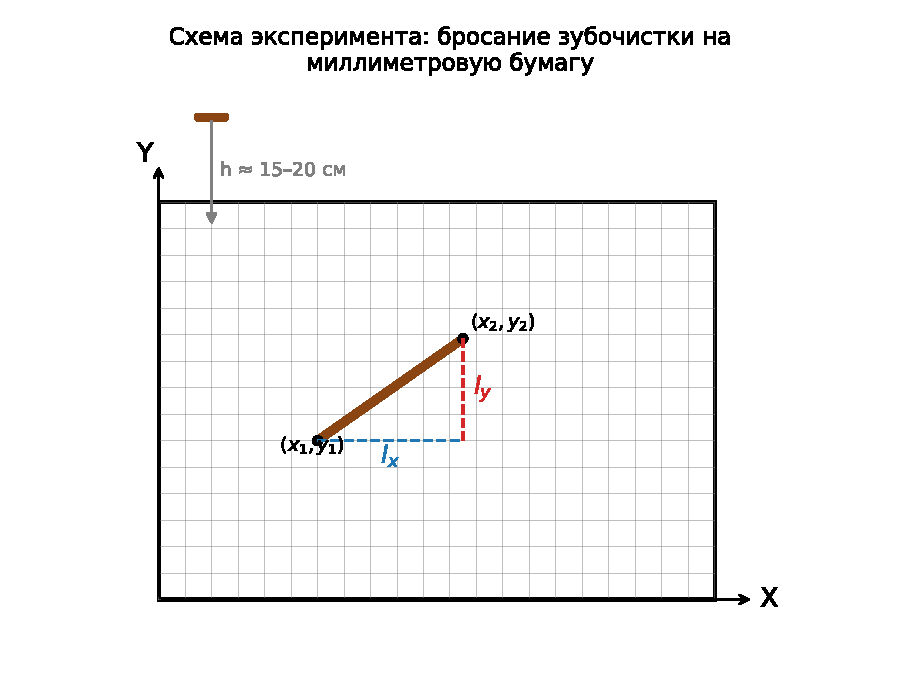
\includegraphics[width=0.62\linewidth]{scheme.pdf}
  \caption{Схема эксперимента: бросание зубочистки на миллиметровую бумагу.
    Показаны оси $X$ и $Y$, направление свободного падения зубочистки
    с высоты $h$, а также определяемые по координатам концов зубочистки
  модули проекций $l_x$ и $l_y$.}
  \label{fig:scheme}
\end{figure}

\phantomsection
\section*{Краткое теоретическое введение}
\addcontentsline{toc}{section}{Краткое теоретическое введение}

Зубочистка длиной $L$ падает на плоскость случайным образом. Ее положение
задается углом $\varphi$ между зубочисткой и осью $X$. Куда именно
направлена зубочистка --- не имеет значения, все четыре четверти плоскости
равноправны, поэтому будем считать что угол $\varphi$ равновероятно принимает
любое значение из $[0, \ \pi/2]$.

При фиксированном угле проекции равны
\begin{equation}
  l_x = L \cos\varphi, \qquad
  l_y = L \sin\varphi.
  \label{eq:proj}
\end{equation}

Раз $\varphi$ распределен равномерно, среднее по всем углам --- это просто
среднее интегральное по промежутку $[0,\ \pi/2)$, деленное на его длину:
\begin{equation}
  \langle l_x \rangle
  = \frac{2}{\pi}\int\limits_{0}^{\pi/2} L\cos\varphi\,d\varphi
  = \frac{2L}{\pi},
  \label{eq:mean_lx}
\end{equation}
\begin{equation}
  \langle l_y \rangle
  = \frac{2}{\pi}\int\limits_{0}^{\pi/2} L\sin\varphi\,d\varphi
  = \frac{2L}{\pi}.
  \label{eq:mean_ly}
\end{equation}

Средние проекции совпадают. Тогда
\begin{equation}
  A_{\text{теор}} = \frac{L}{\langle l_x \rangle} = \frac{\pi}{2}
  \approx 1{,}5708,
  \qquad
  B_{\text{теор}} = \frac{L}{\langle l_y \rangle} = \frac{\pi}{2}
  \approx 1{,}5708.
  \label{eq:AB_theor}
\end{equation}

То есть по модели $A$ и $B$ должны быть равны друг другу и равны $\pi/2$,
причем независимо от длины зубочистки и высоты броска. Число $\pi$ известно
с любой нужной точностью, так что погрешность самого теоретического
значения $\pi/2$ на практике равна нулю; все отклонение экспериментальных
и модельных $A$, $B$ от $\pi/2$ --- это конечность выборки и точность измерений.

\phantomsection
\section*{Полученные экспериментальные данные}
\addcontentsline{toc}{section}{Полученные экспериментальные данные}

Было проведено $n = 50$ бросков зубочистки на миллиметровую бумагу. Для
каждого броска модули проекций на оси $X$ и $Y$ фиксировались с точностью
до целого миллиметра --- цена деления миллиметровки не позволяет точнее.
Результаты --- в таблице~\ref{tab:raw_data}.

\begin{table}[H]
  \centering
  \caption{Результаты измерений модулей проекций зубочистки $l_x$ и $l_y$, мм}
  \label{tab:raw_data}
  \begin{tabular}{|c|c|c|c|c|c|}
    \hline
    № & $l_x$, мм & $l_y$, мм & № & $l_x$, мм & $l_y$, мм \\
    \hline
    1 & 33 & 58 & 26 & 38 & 56 \\
    \hline
    2 & 62 & 26 & 27 & 29 & 60 \\
    \hline
    3 & 42 & 53 & 28 & 44 & 52 \\
    \hline
    4 & 52 & 42 & 29 & 11 & 66 \\
    \hline
    5 & 42 & 51 & 30 & 67 &  7 \\
    \hline
    6 & 22 & 64 & 31 &  6 & 66 \\
    \hline
    7 & 64 & 19 & 32 & 22 & 63 \\
    \hline
    8 & 21 & 63 & 33 & 12 & 66 \\
    \hline
    9 & 49 & 46 & 34 & 60 & 29 \\
    \hline
    10 & 67 &  5 & 35 & 63 & 25 \\
    \hline
    11 & 37 & 56 & 36 & 19 & 64 \\
    \hline
    12 & 62 & 25 & 37 & 45 & 50 \\
    \hline
    13 & 65 & 17 & 38 & 42 & 53 \\
    \hline
    14 &  6 & 67 & 39 & 37 & 56 \\
    \hline
    15 & 53 & 42 & 40 & 21 & 63 \\
    \hline
    16 & 66 & 12 & 41 & 36 & 57 \\
    \hline
    17 & 65 & 11 & 42 & 48 & 46 \\
    \hline
    18 & 29 & 60 & 43 & 23 & 61 \\
    \hline
    19 & 22 & 63 & 44 & 66 &  5 \\
    \hline
    20 & 47 & 48 & 45 & 60 & 29 \\
    \hline
    21 & 49 & 46 & 46 & 44 & 50 \\
    \hline
    22 & 67 &  6 & 47 & 15 & 65 \\
    \hline
    23 & 47 & 47 & 48 & 54 & 40 \\
    \hline
    24 & 48 & 46 & 49 & 15 & 65 \\
    \hline
    25 & 19 & 64 & 50 & 51 & 49 \\
    \hline
  \end{tabular}
\end{table}

\phantomsection
\section*{Статистическая обработка полученных результатов}
\addcontentsline{toc}{section}{Статистическая обработка полученных результатов}

Все расчеты в этом разделе сделаны программой на C++.

Средние арифметические значения модулей проекций вычисляются по формулам
\begin{equation}
  \langle l_x \rangle = \frac{1}{n}\sum_{i=1}^{n} l_{x_i},
  \qquad
  \langle l_y \rangle = \frac{1}{n}\sum_{i=1}^{n} l_{y_i},
\end{equation}
где $n = 50$ --- число измерений, $l_{x_i}$ и $l_{y_i}$ --- результаты отдельных измерений, взятые из таблицы~\ref{tab:raw_data}.

Подстановка данных из таблицы дает:
\[
  \langle l_x \rangle = 41{,}28\,\text{мм},
  \qquad
  \langle l_y \rangle = 45{,}60\,\text{мм}.
\]

Случайная погрешность многократных равноточных измерений рассчитывается по формуле
\begin{equation}
  \Delta l_{x\,\text{сл}}
  = k_{\alpha,n}
  \sqrt{\frac{\sum\limits_{i=1}^{n}
  \bigl(l_{x_i} - \langle l_x \rangle\bigr)^2}{n(n-1)}},
  \label{eq:rand_err}
\end{equation}
где $k_{\alpha,n}$ --- коэффициент Стьюдента для доверительной вероятности
$\alpha = 0{,}95$ и числа измерений $n = 50$; по таблице коэффициентов
Стьюдента $k_{0{,}95;\,50} = 2{,}0$. Для $\Delta l_{y\,\text{сл}}$ --- та же формула.

Полная погрешность среднего складывается из случайной и инструментальной по формуле:
\begin{equation}
  \Delta l_x
  = \sqrt{\bigl(\Delta l_{x\,\text{сл}}\bigr)^2 + \bigl(\Delta l_{\text{инстр}}\bigr)^2}.
  \label{eq:tot_err}
\end{equation}

$\Delta l_y$ считаем так же.

Погрешности проекций в результате выходят следующими:
\begin{align*}
  \Delta l_{x\,\text{сл}} &= 5{,}28\,\text{мм}, &
  \Delta l_x &= 5{,}30\,\text{мм}, \\
  \Delta l_{y\,\text{сл}} &= 5{,}46\,\text{мм}, &
  \Delta l_y &= 5{,}48\,\text{мм}.
\end{align*}

Длина зубочистки была измерена линейкой с ценой деления $1\,\text{мм}$:
\[
  L = (67{,}0 \pm 0{,}5)\,\text{мм}.
\]

$A$ и $B$ --- косвенные измерения, их погрешности находим по формулам
\begin{equation}
  A = \frac{L}{\langle l_x \rangle},
  \qquad
  \Delta A = A\sqrt{\left(\frac{\Delta L}{L}\right)^2 + \left(\frac{\Delta l_x}{\langle l_x \rangle}\right)^2},
  \label{eq:A}
\end{equation}
\begin{equation}
  B = \frac{L}{\langle l_y \rangle},
  \qquad
  \Delta B = B\sqrt{\left(\frac{\Delta L}{L}\right)^2 + \left(\frac{\Delta l_y}{\langle l_y \rangle}\right)^2}.
  \label{eq:B}
\end{equation}

Подстановка чисел дает окончательный результат:
\[
  A = (1{,}62 \pm 0{,}21),
  \qquad
  B = (1{,}47 \pm 0{,}18).
\]

Относительные погрешности:
\[
  \varepsilon_A = \frac{\Delta A}{A} \approx 0{,}13 \quad (13\,\%),
  \qquad
  \varepsilon_B = \frac{\Delta B}{B} \approx 0{,}12 \quad (12\,\%).
\]

$A$ и $B$ перекрываются друг с другом и с теоретическим $\pi/2 \approx 1{,}5708$
в пределах погрешности: $A$ отклоняется от $\pi/2$ всего на $\approx 0{,}05$
при $\Delta A = 0{,}21$, $B$ --- на $\approx 0{,}10$ при $\Delta B = 0{,}18$.
Эксперимент согласуется с теорией.

\phantomsection
\section*{Численное моделирование}
\addcontentsline{toc}{section}{Численное моделирование}

Для проверки модели и оценки необходимого числа опытов эксперимент был
промоделирован методом Монте-Карло. Угол $\varphi$ генерировался как
равномерная случайная величина на $[0,\ \pi/2)$, после чего по
формуле~\eqref{eq:proj} для каждого $\varphi_i$ вычислялись
$l_{x_i} = L\cos\varphi_i$ и $l_{y_i} = L\sin\varphi_i$ при
$L = 67{,}0\,\text{мм}$. Для каждого $n$ находились средние $\langle l_x\rangle$,
$\langle l_y\rangle$, стандартная ошибка среднего и отношения
$A = L/\langle l_x\rangle$, $B = L/\langle l_y\rangle$. Моделирование
выполнено на языке C++, генератор псевдослучайных чисел --- стандартный.

Результаты для разных $n$ --- в таблице~\ref{tab:sim}.

\begin{table}[H]
  \centering
  \caption{Результаты численного моделирования при различном числе опытов $n$}
  \label{tab:sim}
  \begin{tabular}{|c|c|c|c|c|}
    \hline
    $n$ & $\langle l_x\rangle$, мм & $\langle l_y\rangle$, мм & $A$ & $B$ \\
    \hline
    30      & 42{,}92 & 41{,}25 & 1{,}561 & 1{,}624 \\
    \hline
    50      & 44{,}24 & 40{,}42 & 1{,}514 & 1{,}658 \\
    \hline
    100     & 41{,}41 & 43{,}67 & 1{,}618 & 1{,}534 \\
    \hline
    500     & 43{,}62 & 41{,}97 & 1{,}536 & 1{,}597 \\
    \hline
    1000    & 41{,}20 & 43{,}74 & 1{,}626 & 1{,}532 \\
    \hline
    5000    & 42{,}79 & 42{,}85 & 1{,}566 & 1{,}564 \\
    \hline
    10000   & 42{,}61 & 42{,}58 & 1{,}572 & 1{,}574 \\
    \hline
  \end{tabular}
\end{table}

При малых $n$ ($\lesssim 100$) $A$ и $B$ заметно колеблются вокруг $\pi/2$
и заметно отличаются друг от друга --- обычный разброс малой выборки, тот же,
что и в реальном эксперименте при $n=50$. К $n \sim 10^3$--$10^4$ оба значения
сходятся к $\pi/2$ уже до третьего знака, что подтверждает модель. Сходимость
$A(n)$ и $B(n)$ показана на рисунке~\ref{fig:convergence}.

\begin{figure}[H]
  \centering
  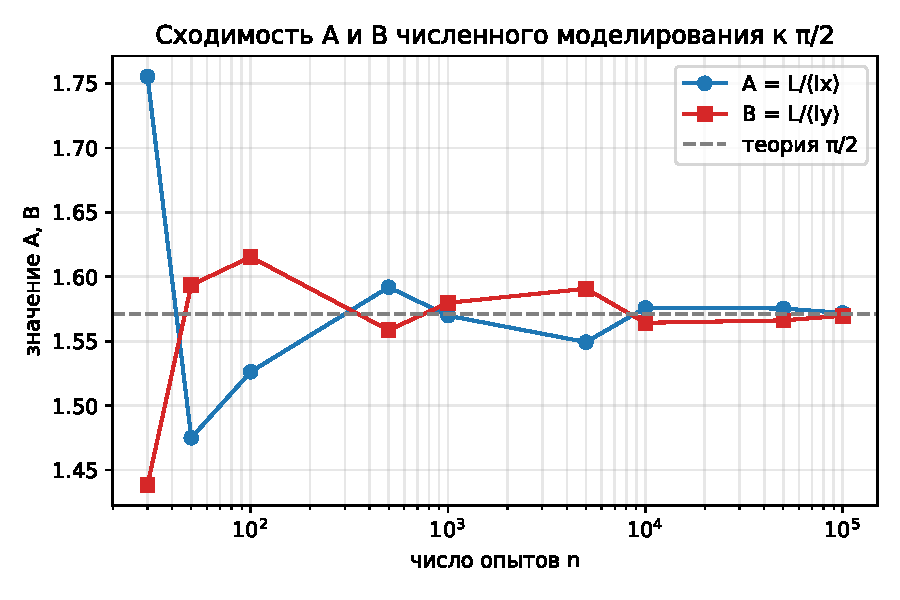
\includegraphics[width=0.75\linewidth]{convergence.pdf}
  \caption{Сходимость значений $A$ и $B$, полученных путем численного
    моделирования, к теоретическому значению $\pi/2$ при увеличении
  числа опытов $n$ (логарифмическая шкала по оси $n$).}
  \label{fig:convergence}
\end{figure}

Погрешность среднего $\sigma/\sqrt{n}$ падает как $1/\sqrt{n}$: рост $n$
в 100 раз (с $10^2$ до $10^4$) дает выигрыш в точности примерно в 10 раз ---
при $n=1000$ погрешность среднего $\approx 0{,}6\,\text{мм}$, при $n=10000$
--- уже $\approx 0{,}2\,\text{мм}$. Для точности порядка $1\,\%$ требуется
порядка $10^4$ бросков, что практически нереализуемо вручную. При этом для
реального эксперимента дальнейшее увеличение $n$ не дает существенного
выигрыша: приборная погрешность считывания координат ($0{,}5\,\text{мм}$)
уже при $n\sim50$ сравнима со случайной, и рост $n$ почти не уменьшает
полную погрешность. Поэтому 50 бросков --- разумный компромисс между
точностью и затраченным временем.

Сравнение всех трех результатов --- в таблице~\ref{tab:compare}.

\begin{table}[H]
  \centering
  \caption{Сравнение значений $A$ и $B$, полученных разными методами}
  \label{tab:compare}
  \begin{tabular}{|l|c|c|}
    \hline
    Метод & $A$ & $B$ \\
    \hline
    Эксперимент ($n=50$) & $1{,}62 \pm 0{,}21$ & $1{,}47 \pm 0{,}18$ \\
    \hline
    Теория & \multicolumn{2}{c|}{$\pi/2 \approx 1{,}5708$} \\
    \hline
    Численное моделирование ($n=10^4$) & $1{,}572$ & $1{,}574$ \\
    \hline
  \end{tabular}
\end{table}

Эксперимент, теория и моделирование дают согласующиеся значения $A$ и $B$ ---
модель равномерного угла падения зубочистки описывает явление верно.

\phantomsection
\section*{Заключение}
\addcontentsline{toc}{section}{Заключение}

Модель равномерного угла падения зубочистки предсказывает
$A_{\text{теор}} = B_{\text{теор}} = \pi/2 \approx 1{,}5708$ независимо от
длины зубочистки. В эксперименте ($n=50$) получено
\[
  A = 1{,}62 \pm 0{,}21, \qquad B = 1{,}47 \pm 0{,}18,
\]
оба значения согласуются с теоретическим $\pi/2$ в пределах погрешности.

Численное моделирование при $n \gtrsim 10^3$ также сходится к $\pi/2$, а при
$n=50$ даёт такой же разброс, как и реальный эксперимент --- то есть
расхождение $A$ и $B$ между собой объясняется не ошибкой методики, а
статистикой малой выборки.

Погрешность результата определяется в основном случайным разбросом
$l_x$, $l_y$ ($\approx5{,}3$--$5{,}5\,\text{мм}$); приборная погрешность
миллиметровки ($0{,}5\,\text{мм}$) на этом фоне пренебрежимо мала. Значит,
точность имеет смысл повышать увеличением числа бросков, а не более
точной линейкой: по модели, для уменьшения погрешности в 2 раза нужно
около 200 бросков, а для точности в $1\,\%$ --- порядка $10^4$, что
практически нереализуемо вручную.

Цель работы выполнена: эксперимент, теория и моделирование дают согласующиеся
значения $A$ и $B$.

\end{document}